\chapter{Specifikacija programske potpore}
	\section{Funkcionalni zahtjevi}
			\noindent \textbf{Dionici:}
			\begin{packed_enum}
				\item Roditelj
				\item Pedijatar
                \item Liječnik obiteljske medicine
                \item Administrator
			\end{packed_enum}
			
			\noindent \textbf{Aktori i njihovi funkcionalni zahtjevi:}
			\begin{packed_enum}
				\item  \underbar{Roditelj (inicijator) može:}
				\begin{packed_enum}
					\item registrirati se i prijaviti u sustav
                    \item vidjeti profil za sebe i svoju djecu
					\item pregledati medicinske nalaze, dijagnoze i povijesti pregleda za sebe i svoju djecu
					\item unijeti nalaz dobiven na temelju određenog pregleda ili postupka u privatnoj ustanovi te zatražiti drugo mišljenje liječnika ili pedijatra
                    \item vidjeti zahtjeve za drugim mišljenjima koje je stvorio
                    \item vidjeti upute koje su on ili njegova djeca dobili od liječnika/pedijatra
				\end{packed_enum}
			
				\item  \underbar{Pedijatar (inicijator) može:}
				\begin{packed_enum}
					\item prijaviti se u sustav
                    \item prijaviti djecu po identifikatoru (OIB)
                    \item pregledati popis sve prijavljene djece i njihove kartone
					\item unijeti medicinske podatke (dijagnoze, preglede, terapije)
                    \item evidentirati preporuku za bolovanje za roditelja u slučaju bolesti djeteta
                    \item utvrditi bolest djeteta nakon čega se šalje ispričnica u vrtić
                    \item naručiti djecu na specijalističke preglede/postupke
                    \item izdati uputu pacijentu
                    \item dati drugo mišljenje
				\end{packed_enum}

                \item  \underbar{Liječnik obiteljske medicine (inicijator) može:}
				\begin{packed_enum}
					\item prijaviti se u sustav
                    \item pregledati i odobriti preporuke za bolovanje izdane od strane pedijatra 
					\item slati doznake za bolovanje poslodavcu roditelja
					\item izdati uputu pacijentu
                    \item dati drugo mišljenje
                    \item naručiti pacijenta na specijalistički pregled/postupak
                    \item unositi podatke o pregledima
                    \item pristupiti medicinskim nalazima, povijesti pregleda i upitima 
				\end{packed_enum}
    
                \item  \underbar{Administrator (inicijator) može:}
				\begin{packed_enum}
                    \item prijaviti se u sustav kao administrator
					\item pripremiti registre djece (ime, prezime, OIB)
                    \item registrirati liječnika obiteljske medicine i pedijatra
                    \item po registraciji roditelja, povezati iste s djecom (preko OIB-a)
					\item administrirati korisničke račune
                    \item ažurirati sve podatke u aplikaciji
				\end{packed_enum}

                \item  \underbar{Baza podataka (sudionik):}
				\begin{packed_enum}
                    \item pohranjuje sve podatke o korisnicima i njihovim ovlastima
				\end{packed_enum}
			\end{packed_enum}
			
			\eject 
				
			\subsection{Obrasci uporabe}
				
				%dio 1. revizije
				
				\subsubsection{Opis obrazaca uporabe}
					%Funkcionalne zahtjeve razraditi u obliku obrazaca uporabe. Ukoliko u nekom koraku može doći do odstupanja, potrebno je to odstupanje opisati i po mogućnosti ponuditi rješenje kojim bi se tijek obrasca vratio na osnovni tijek.
					

					\noindent \underbar{\textbf{UC1 - registriraj se}}
					\begin{packed_item}
	
						\item \textbf{Glavni sudionik: }korisnik
						\item  \textbf{Cilj:} stvoriti korisnički račun za pristup sustavu
						\item  \textbf{Sudionici:} baza podataka
						\item  \textbf{Preduvjet:} korisnik je otvorio početnu stranicu za registraciju u aplikaciju
						\item  \textbf{Opis osnovnog tijeka:}
						
						\item[] \begin{packed_enum}
							\item korisnik odabire opciju registriraj se
							\item sustav otvara ekran registracije
							\item korisnik unosi potrebne korisničke podatke
							\item korisnik potvrđuje unos podataka odabirom akcije potvrdi
							\item sustav provjerava i utvrđuje da je unos uspješan
							\item sustav obavještava korisnika o uspješnoj registraciji

						\end{packed_enum}
						
						\item  \textbf{Opis mogućih odstupanja:}
						
						\item[] \begin{packed_item}
							\item[4.a] Korisnik odustaje od unosa podatka (odabir akcije odustani)
							\item[] \begin{packed_enum}
								
								\item sustav zatvara trenutni ekran
								\item izvođenje scenarija je završeno
							\end{packed_enum}
							\item[5.a] Odabir već zauzetog korisničkog imena i/ili e-maila, unos korisničkih podatka u nedozvoljenom formatu
							\item[] \begin{packed_enum}
								
								\item sustav obavještava korisnika o neuspjelom upisu
								\item sustav nastavlja izvođenje u koraku 3
							\end{packed_enum}
							
						\end{packed_item}
					\end{packed_item}

                    \noindent \underbar{\textbf{UC2 - prijavi se}}
					\begin{packed_item}
	
						\item \textbf{Glavni sudionik: }korisnik
						\item  \textbf{Cilj: }dobiti pristup korisničkom sučelju
						\item  \textbf{Sudionici: }baza podataka
						\item  \textbf{Preduvjet: } izvođenje UC1
						\item  \textbf{Opis osnovnog tijeka:}
						
						\item[] \begin{packed_enum}
							\item korisniku se po upisu web adrese aplikacije otvara početna stranica
							\item korisnik odabire akciju 'Prijavi se'
							\item sustav otvara ekran prijave
							\item korisnik unosi email i lozinku
							\item korisnik odabire akciju potvrde unosa
							\item sustav provjerava i utvrđuje da je unos uspješan
							\item korisniku se prikazuje početni zaslon aplikacije

						\end{packed_enum}
						
						\item  \textbf{Opis mogućih odstupanja:}
						
						\item[] \begin{packed_item}
							\item[5.a] Korisnik odabire akciju 'Odustani'
							\item[] 
							\begin{packed_enum} 
								\item sustav zatvara ekran
								\item prikazuje se prethodni ekran i završava izvođenje ovog scenarija
							\end{packed_enum}
							\item[6.a]  sustav provjerava i utvrđuje da unos podataka nije uspješan
							\item[] 
							\begin{packed_enum}
								\item sustav obavještava korisnika porukom na modalnom ekranu o unosu pogrešne lozinke
								\item sustav nastavlja izvođenje u koraku 4. (korisnik ispravlja unesenu lozinku i dalje scenarij ide svojim tijekom)
							\end{packed_enum}
							
						\end{packed_item}
					\end{packed_item}

                    \noindent \underbar{\textbf{UC3 - pregledaj profil djeteta}}
					\begin{packed_item}
	
						\item \textbf{Glavni sudionik: }roditelj
						\item  \textbf{Cilj:} pregledati djetetovu povijest pregleda, nalaze i dijagnoze
						\item  \textbf{Sudionici:} baza podataka
						\item  \textbf{Preduvjet:} izvođenje UC2 i UC22, korisnik ima dijete
						\item  \textbf{Opis osnovnog tijeka:}
						
						\item[] \begin{packed_enum}
		
							\item roditelj odabire opciju 'Moja djeca' na početnoj stranici
							\item sustav prikazuje popis djece koja su povezana s roditeljem
							\item roditelj odabire dijete čije podatke želi pregledati
							\item sustav prikazuje početnu stranicu djetetovog profila
							
						\end{packed_enum}
						
					\end{packed_item}

					\noindent \underbar{\textbf{UC4 - pregledaj povijest pregleda svojeg djeteta}}
					\begin{packed_item}
	
						\item \textbf{Glavni sudionik: }roditelj
						\item  \textbf{Cilj:} pristupiti povijesti pregleda djeteta, za svaki pregled su vidljivi nalazi i dijagnoze ustanovljene na pregledu
						\item  \textbf{Sudionici:} baza podataka
						\item  \textbf{Preduvjet:} izvođenje UC2, UC23
						\item  \textbf{Opis osnovnog tijeka:}
						
						\item[] \begin{packed_enum}
	
							\item roditelj odabire opciju 'Moji pregledi' s početne stranice
							\item sustav prikazuje popis svih obavljenih i zakazanih pregleda korisnika i njegove djece
							\item korisnik filtrira popis pregleda tako da vidi samo djetetove preglede
							\item sustav prikazuje filtrirani popis pregleda
							\item korisnik odabire pregled za koji želi vidjeti podatke
							\item sustav prikazuje podatke o odabranom pregledu
							
						\end{packed_enum}
						\item  \textbf{Opis mogućih odstupanja:}
						
						\item[] \begin{packed_item}
							\item[2.a] korisnik nema nijedan zabilježeni pregled
							\item[] 
							\begin{packed_enum} 
								\item prikazuje se poruka 'Ne postoji nijedan zabilježeni pregled'
								\item završava izvođenje ovog scenarija
								
							\end{packed_enum}
						\end{packed_item}
					\end{packed_item}

                    
                    \noindent \underbar{\textbf{UC5 - pregledaj vlastiti profil}}
					\begin{packed_item}
	
						\item \textbf{Glavni sudionik: }korisnik
						\item  \textbf{Cilj:} pregledati vlastiti profil
						\item  \textbf{Sudionici:} baza podataka
						\item  \textbf{Preduvjet:} izvođenje UC2
						\item  \textbf{Opis osnovnog tijeka:}
						
						\item[] \begin{packed_enum}
	
							\item korisnik odabire opciju 'Moj profil' s početne stranice
							\item sustav prikazuje osobne podatke korisnika 
			
						\end{packed_enum}
						
						
					\end{packed_item}

					\noindent \underbar{\textbf{UC6 - ažuriraj e-mail adresu poslodavca}}
					\begin{packed_item}
	
						\item \textbf{Glavni sudionik: }korisnik
						\item  \textbf{Cilj:} ažurirati e-mail adresu svog poslodavca
						\item  \textbf{Sudionici:} baza podataka
						\item  \textbf{Preduvjet:} izvođenje UC2
						\item  \textbf{Opis osnovnog tijeka:}
						
						\item[] \begin{packed_enum}
	
							\item korisnik odabire opciju 'Profil' s početne stranice
							\item sustav prikazuje osobne podatke korisnika 
							\item korisnik pronalazi polje za unos e-mail adrese poslodavca
							\item korisnik unosi e-mail adresu poslodavca
							\item korisnik odabire opciju 'Spremi promjene'
							\item sustav provjerava i utvrđuje da je unos uspješan
							\item sustav obavještava korisnika da je unos uspješan
			
						\end{packed_enum}
						
						\item  \textbf{Opis mogućih odstupanja:}
						
						\item[] \begin{packed_item}
							\item[6.a] korisnik je unio pogrešnu e-mail adresu 
							\item[] 
							\begin{packed_enum} 
								\item prikazuje se poruka 'Pogrešan unos e-mail adrese'
								\item sustav vraća korisnika na ponovno upisivanje e-mail adrese
								\item scenarij se nastavlja od koraka 4
								
							\end{packed_enum}
						\end{packed_item}
						
					\end{packed_item}

					\noindent \underbar{\textbf{UC7 - ažuriraj e-mail adresu vrtića/škole}}
					\begin{packed_item}
	
						\item \textbf{Glavni sudionik: }roditelj
						\item  \textbf{Cilj:} ažurirati e-mail adresu djetetovog vrtića/škole
						\item  \textbf{Sudionici:} baza podataka
						\item  \textbf{Preduvjet:} izvođenje UC2 i UC22
						\item  \textbf{Opis osnovnog tijeka:}
						
						\item[] \begin{packed_enum}
							\item roditelj odabire opciju 'Moja djeca' s početne stranice
							\item sustav prikazuje popis djece koja su povezana s roditeljem
							\item roditelj odabire dijete čije podatke želi ažurirati
							\item sustav prikazuje osobne podatke o djetetu
							\item roditelj pronalazi polje za unos e-mail adrese vrtića/škole
							\item roditelj unosi e-mail adresu vrtića/škole
							\item roditelj odabire opciju 'Spremi promjene'
							\item sustav provjerava i utvrđuje da je unos uspješan
							\item sustav obavještava roditelja da je unos uspješan
			
						\end{packed_enum}
						
						\item  \textbf{Opis mogućih odstupanja:}
						
						\item[] \begin{packed_item}
							\item[8.a] roditelj je unio pogrešnu e-mail adresu 
							\item[] 
							\begin{packed_enum} 
								\item prikazuje se poruka 'Pogrešan unos e-mail adrese'
								\item sustav vraća roditelja na ponovno upisivanje e-mail adrese
								\item scenarij se nastavlja od koraka 6
								
							\end{packed_enum}
						\end{packed_item}
						
					\end{packed_item}


                     \noindent \underbar{\textbf{UC8 - pregledaj medicinske podatke}}
					\begin{packed_item}
	
						\item \textbf{Glavni sudionik: }korisnik
						\item  \textbf{Cilj:} pristupiti povijesti pregleda, za svaki pregled su vidljivi nalazi i dijagnoze ustanovljene na pregledu
						\item  \textbf{Sudionici:} baza podataka
						\item  \textbf{Preduvjet:} izvođenje UC2
						\item  \textbf{Opis osnovnog tijeka:}
						
						\item[] \begin{packed_enum}
	
							\item roditelj odabire opciju 'Moji pregledi' s početne stranice
							\item sustav prikazuje popis svih obavljenih i zakazanih pregleda
							\item korisnik odabire pregled za koji želi vidjeti podatke
							\item sustav prikazuje podatke o odabranom pregledu
							
						\end{packed_enum}
						\item  \textbf{Opis mogućih odstupanja:}
						
						\item[] \begin{packed_item}
							\item[2.a] korisnik nema nijedan zabilježeni pregled
							\item[] 
							\begin{packed_enum} 
								\item prikazuje se poruka 'Ne postoji nijedan zabilježeni pregled'
								\item završava izvođenje ovog scenarija
								
							\end{packed_enum}
						\end{packed_item}
					\end{packed_item}

                    \noindent \underbar{\textbf{UC9 - stvori zahtjev za drugim mišljenjem}}
					\begin{packed_item}
						\item \textbf{Glavni sudionik: }korisnik
						\item  \textbf{Cilj:} zatražiti drugo mišljenja liječnika ili pedijatra o nalazu dobivenom na temelju određene usluge u privatnoj ustanovi
						\item  \textbf{Sudionici:} baza podataka
						\item  \textbf{Preduvjet:} izvođenje UC2, pacijent ima dodijeljenog liječnika ili pedijatra
						\item  \textbf{Opis osnovnog tijeka:}
						
						\item[] \begin{packed_enum}
							\item korisnik odabire opciju 'Zatraži drugo mišljenje'
							\item sustav otvara modalni okvir unosa zahtjeva za drugim mišljenjem
							\item roditelj prenosi nalaz dobiven u privatnoj ustanovi
                            \item roditelj odabire liječnika/pedijatra čije drugo mišljenje želi dobiti
							\item roditelj odabire akciju 'Pošalji zahtjev'
							\item sustav provjerava i utvrđuje da je unos uspješan
							\item prikazuje se poruka 'Zahtjev uspješno poslan'
						
						\end{packed_enum}
						
						\item  \textbf{Opis mogućih odstupanja:}
						
						\item[] \begin{packed_item}
                            \item[5.a] neispravno popunjen zahtjev
                            \item[] \begin{packed_enum}
                            	\item sustav utvrđuje da je zahtjev neispravno popunjen
								\item sustav usmjerava korisnika na ponovno ispunjavanje zahtjeva za drugim mišljenjem
								\item nakon ispravnog unosa, korisnik odabire akciju 'Pošalji zahtjev' te se scenarij nastavlja od koraka 6
							\end{packed_enum}
							\item[5.b] korisnik odabire akciju 'Odustani'
                            \item[] \begin{packed_enum}
                            	\item sustav zatvara modalni ekran
								\item prikazuje se prethodni ekran i završava izvođenje ovog scenarija
							\end{packed_enum}
						\end{packed_item}
					\end{packed_item}


                    \noindent \underbar{\textbf{UC10 - Pregledaj zahtjev za drugim mišljenjem}}
					\begin{packed_item}
	
						\item \textbf{Glavni sudionik: }korisnik
						\item  \textbf{Cilj:} pregledati predani zahtjev za drugim mišljenjem te liječnikovu ili pedijatrovu povratnu informaciju 
						\item  \textbf{Sudionici:} baza podataka
						\item  \textbf{Preduvjet:} izvođenje UC2 i UC9
						\item  \textbf{Opis osnovnog tijeka:}
						
						\item[] \begin{packed_enum}
	
							\item korisnik odabire opciju 'Moji zahtjevi' s početne stranice
							\item sustav prikazuje popis svih korisnikovih zahtjeva za drugim mišljenjem
							\item korisnik odabire zahtjev koji želi pregledati
                            \item sustav prikazuje korisnikov zahtjev za drugim mišljenjem
                            \item korisnik pregledava liječnikov odgovor na zahtjev

						\end{packed_enum}
						
						\item  \textbf{Opis mogućih odstupanja:}
						
						\item[] \begin{packed_item}
	
							\item[5.a] liječnik nije poslao svoje drugo mišljenje
							\item[] \begin{packed_enum}
								\item roditelj može vidjeti samo svoj predani zahtjev
								\item sustav prikazuje poruku 'Liječnik nije poslao svoje drugo mišljenje!' u polju za odgovor liječnika
								\item završava se izvođenje ovog scenarija 
							\end{packed_enum}
							
						\end{packed_item}
					\end{packed_item}

                    \noindent \underbar{\textbf{UC11 - prijavi pacijenta u svoju ordinaciju }}
					\begin{packed_item}
	
						\item \textbf{Glavni sudionik: }pedijatar, liječnik obiteljske medicine
						\item  \textbf{Cilj:} prijaviti pacijenta u svoju ordinaciju
						\item  \textbf{Sudionici:} baza podataka
						\item  \textbf{Preduvjet:} izvođenje UC2
						\item  \textbf{Opis osnovnog tijeka:}
						
						\item[] \begin{packed_enum}
							\item liječnik odabire opciju 'Pacijenti' s početne stranice
							\item liječnik odabire opciju 'Prijavi pacijenta' s početne stranice
							\item sustav prikazuje popis pacijenata koji nemaju pridijeljenog liječnika
							\item liječnik odabire pacijenta koji postaje njegov pacijent odabirom akcije 'Odaberi pacijenta'
							\item sustav obavještava liječnika da je pacijent uspješno odabran i prijavljen u njegovu ordinaciju

						\end{packed_enum}
						
						\item  \textbf{Opis mogućih odstupanja:}
						
						\item[] \begin{packed_item}
	
							\item[3.a] ne postoji nijedan pacijent koji nema pridijeljenog liječnika
							\item[] \begin{packed_enum}
								\item sustav umjesto popisa pacijenata, prikazuje poruku 'Svi pacijenti imaju pridijeljenog liječnika'
							\end{packed_enum}
							\item[4.a] liječnik odustaje od prijave pacijenta
							\item[] \begin{packed_enum}
								\item sustav zatvara trenutni ekran
								\item završava se izvođenje ovog scenarija
							\end{packed_enum}
							
						\end{packed_item}
					\end{packed_item}

     
                    \noindent \underbar{\textbf{UC12 - pregledaj prijavljene pacijente i  njihove kartone }}
					\begin{packed_item}
	
						\item \textbf{Glavni sudionik: }pedijatar, liječnik obiteljske medicine
						\item  \textbf{Cilj:} pregledati popis prijavljenih pacijenata i njihovih kartona
						\item  \textbf{Sudionici:} baza podataka
						\item  \textbf{Preduvjet:} izvođenje UC2
						\item  \textbf{Opis osnovnog tijeka:}
						
						\item[] \begin{packed_enum}
	
							\item liječnik odabire opciju 'Pacijenti' s početne stranice
							\item sustav prikazuje popis pacijenata koji su prijavljeni u liječnikovoj ordinaciji
							\item liječnik odabire pacijenta čiji karton želi pregledati i odabire opciju 'Pregledaj karton'
							\item sustav prikazuje medicinske podatke o odabranom pacijentu
						\end{packed_enum}
						
						\item  \textbf{Opis mogućih odstupanja:}
						
						\item[] \begin{packed_item}
	
							\item[2.a] liječnik nema nijednog pacijenta
							\item[] \begin{packed_enum}
								
								\item sustav prikazuje poruku 'Nemate nijednog prijavljenog pacijenta'
								\item završava se izvođenje ovog scenarija
							\end{packed_enum}
							
						\end{packed_item}
					\end{packed_item}


                    \noindent \underbar{\textbf{UC13 - unesi pregled}}
					\begin{packed_item}
	
						\item \textbf{Glavni sudionik: }pedijatar, liječnik obiteljske medicine
						\item  \textbf{Cilj:} unijeti pregled te medicinske podatke vezane uz pregled: dijagnoza, nalaz, terapija
						\item  \textbf{Sudionici:} baza podataka
						\item  \textbf{Preduvjet:} izvođenje UC2 i UC11
						\item  \textbf{Opis osnovnog tijeka:}
						
						\item[] \begin{packed_enum}
							\item liječnik odabire opciju 'Pregledi' s početne stranice
							\item liječnik odabire opciju 'Novi pregled' s početne stranice
							\item sustav prikazuje modalni ekran za unos pregleda
							\item liječnik odabire pacijenta iz padajućeg izbornika za kojega želi unijeti novi pregled
							\item liječnik unosi podatke o pregledu
							\item liječnik odabire opciju 'Unesi pregled'
							\item sustav provjerava i utvrđuje da je unos uspješan
							\item sustav obavještava liječnika da je pregled uspješno unesen

						\end{packed_enum}

						\item  \textbf{Opis mogućih odstupanja:}
						
						\item[] \begin{packed_item}
	
							\item[7.a] liječnik je pogrešno unio podatke o pregledu
							\item[] \begin{packed_enum}
								
								\item sustav prikazuje poruku 'Neispravan unos podataka o pregledu'
								\item sustav vraća liječnika na izmjenu pogrešnih podataka o pregledu
								\item scenarij se nastavlja od koraka 5
							\end{packed_enum}
							\item [7.b] liječnik odabire opciju 'Odustani'
							\item [] \begin{packed_enum}
								\item sustav zatvara modalni ekran
								\item prikazuje se prethodni ekran i završava izvođenje ovog scenarija
							\end{packed_enum}
						\end{packed_item}
						
					\end{packed_item}

                    \noindent \underbar{\textbf{UC14 - evidentiraj preporuku za bolovanje}}
					\begin{packed_item}
	
						\item \textbf{Glavni sudionik: }pedijatar
						\item  \textbf{Cilj:} evidentirati preporuku za bolovanje roditelja u slučaju bolesti djeteta
						\item  \textbf{Sudionici:} baza podataka
						\item  \textbf{Preduvjet:} izvođenje UC2 i UC13
						\item  \textbf{Opis osnovnog tijeka:}
						
						\item[] \begin{packed_enum}
							\item pedijatar odabire opciju 'Preporuke za bolovanje' s početne stranice
							\item pedijatar odabire opciju 'Nova preporuka za bolovanje' s početne stranice
							\item sustav prikazuje modalni okvir za unos preporuke za bolovanje
							\item pedijatar odabire pregled na temelju kojeg je potrebna preporuka za bolovanje
							\item pedijatar odabire opciju 'Unesi preporuku'
							\item sustav provjerava i potvrđuje da je unos uspješan
							\item sustav obavještava pedijatra da je preporuka uspješno unesena
				
						\end{packed_enum}
						\item  \textbf{Opis mogućih odstupanja:}
						
						\item[] \begin{packed_item}
	
							\item[6.a] liječnik odabire opciju 'Odustani'
							\item [] \begin{packed_enum}
								\item sustav zatvara modalni ekran
								\item prikazuje se prethodni ekran i završava izvođenje ovog scenarija
							\end{packed_enum}
						\end{packed_item}
                    \end{packed_item}
						
                    \noindent \underbar{\textbf{UC15 - pošalji ispričnicu u vrtić/školu}}
					\begin{packed_item}
	
						\item \textbf{Glavni sudionik: }pedijatar
						\item  \textbf{Cilj:} poslati ispričnicu zbog bolesti djeteta u djetetov vrtić/školu
						\item  \textbf{Sudionici:} baza podataka
						\item  \textbf{Preduvjet:} izvođenje UC2 i UC13
						\item  \textbf{Opis osnovnog tijeka:}
						
						\item[] \begin{packed_enum}
							\item pedijatar odabire opciju 'Pregledi' s početne stranice
							\item pedijatar odabire pregled na temelju kojega je potrebno poslati ispričnicu
							\item pedijatar odabire opciju 'Pošalji ispričnicu'
							\item pedijatar unosi podatke o ispričnici
							\item pedijatar odabire opciju pošalji
                            \item sustav provjerava i potvrđuje da je unos uspješan
                            \item sustav obavještava pedijatra da je ispričnica uspješno poslana
						\end{packed_enum}
						
						\item  \textbf{Opis mogućih odstupanja:}
						
						\item[] \begin{packed_item}
	
                            \item[5.a] pedijatar je neispravno popunio ispričnicu
							\item[] \begin{packed_enum}
								\item sustav prikazuje poruku 'Neispravan unos podataka o ispričnici'
								\item pedijatra se vraća na ponovno popunjavanje ispričnice
								\item scenarij se nastavlja od koraka 3
							\end{packed_enum}

							\item[5.b] liječnik odabire opciju 'Odustani'
							\item [] \begin{packed_enum}
								\item sustav zatvara modalni ekran
								\item prikazuje se prethodni ekran i završava izvođenje ovog scenarija
							\end{packed_enum}
							
						\end{packed_item}

						\item \textbf{NAPOMENA:} Iako za ovaj UC postoje sve UI komponente s kojima korisnik ima interakciju, 
						slanje e-maila nije zapravo implementirano jer bi zahtijevalo integraciju sa stvarnim servisima za slanje e-maila.
					\end{packed_item}

     
                    \noindent \underbar{\textbf{UC16 - naruči pacijenta na specijalistički pregled/postupak }}
					\begin{packed_item}
	
						\item \textbf{Glavni sudionik: }pedijatar, liječnik obiteljske medicine
						\item  \textbf{Cilj:} naručiti pacijenta na specijalistički pregled/postupak
						\item  \textbf{Sudionici:} baza podataka
						\item  \textbf{Preduvjet:} izvođenje UC2 i UC11
						\item  \textbf{Opis osnovnog tijeka:}
						
						\item[] \begin{packed_enum}
							
							\item liječnik pregledava popis svojih pacijenata
							\item liječnik odabire pacijenta kojeg želi naručiti na specijalistički pregled/postupak
							\item liječnik stvara novi specijalistički pregled i zakaže vrijeme u budućnosti
                            \item vrijeme i lokacija se šalju pacijentu te je pregled vidljiv pod 'Moji pregledi'

						\end{packed_enum}
						\item  \textbf{Opis mogućih odstupanja:}
						
						\item[] \begin{packed_item}
	
							\item[5.a] liječnik odabire opciju 'Odustani'
							\item [] \begin{packed_enum}
								\item sustav zatvara modalni ekran
								\item prikazuje se prethodni ekran i završava izvođenje ovog scenarija
							\end{packed_enum}
						\end{packed_item}
					\end{packed_item}


                     \noindent \underbar{\textbf{UC17 - prihvati preporuku za bolovanje}}
					\begin{packed_item}
	
						\item \textbf{Glavni sudionik: }liječnik obiteljske medicine
						\item  \textbf{Cilj:} pregledati preporuku za bolovanje roditelja izdanu od strane pedijatra
						\item  \textbf{Sudionici:} baza podataka
						\item  \textbf{Preduvjet:} izvođenje UC2 i UC14
						\item  \textbf{Opis osnovnog tijeka:}
						
						\item[] \begin{packed_enum}
							\item liječnik odabire opciju 'Preporuke za bolovanje' s početne stranice
							\item liječnik pregledava listu preporuka za bolovanje njegovim pacijentima
							\item liječnik odabire preporuku koju želi pregledati
							\item liječnik odabire opciju 'Prihvati' i prihvaća preporuku za bolovanje
                            \item doznaka za bolovanje se šalje poslodavcu pacijenta

						\end{packed_enum}
					\end{packed_item}

					\noindent \underbar{\textbf{UC18 - odbij odluku o preporuci za bolovanje}}
					\begin{packed_item}
	
						\item \textbf{Glavni sudionik: }liječnik obiteljske medicine
						\item  \textbf{Cilj:} pregledati preporuku za bolovanje roditelja izdanu od strane pedijatra
						\item  \textbf{Sudionici:} baza podataka
						\item  \textbf{Preduvjet:} izvođenje UC2 i UC14
						\item  \textbf{Opis osnovnog tijeka:}
						
						\item[] \begin{packed_enum}
							\item liječnik odabire opciju 'Preporuke za bolovanje' s početne stranice
							\item liječnik pregledava listu preporuka za bolovanje njegovim pacijentima
							\item liječnik odabire preporuku koju želi pregledati
							\item liječnik odabire opciju 'Odbij'
                            \item preporuka je odbijena te se ne šalje doznaka za bolovanje poslodavcu pacijenta

						\end{packed_enum}
					\end{packed_item}

					\noindent \underbar{\textbf{UC19 - odjavi se iz sustava}}
					\begin{packed_item}
	
						\item \textbf{Glavni sudionik: }korisnik
						\item  \textbf{Cilj:} odjaviti se iz sustava 
						\item  \textbf{Sudionici:} 
						\item  \textbf{Preduvjet:} izvođenje UC2
						\item  \textbf{Opis osnovnog tijeka:}
						
						\item[] \begin{packed_enum}
							\item korisnik odabire opciju 'Moj profil' s početne stranice
							\item sustav prikazuje korisnički profil
							\item korisnik odabire opciju 'Odjavi se'
							\item sustav odjavljuje korisnika iz sustava i prikazuje početnu stranicu za prijavu

						\end{packed_enum}
					\end{packed_item}
                    
                    \noindent \underbar{\textbf{UC20 - pregledaj korisnika}}
					\begin{packed_item}
	
						\item \textbf{Glavni sudionik: }administrator
						\item  \textbf{Cilj:} pregledati registrirane korisnike
						\item  \textbf{Sudionici:} baza podataka
						\item  \textbf{Preduvjet:} izvođenje UC2
						\item  \textbf{Opis osnovnog tijeka:}
						
						\item[] \begin{packed_enum}
	
							\item administrator odabire opciju 'Korisnici' s početne stranice
							\item sustav prikazuje listu svih korisnika
							\item administrator odabire korisnika čije podatke želi pregledati

						\end{packed_enum}
					\end{packed_item}


                    \noindent \underbar{\textbf{UC21 - promijeni prava pristupa}}
					\begin{packed_item}
	
						\item \textbf{Glavni sudionik: }administrator
						\item  \textbf{Cilj:} promijeniti razinu pristupa korisnika
						\item  \textbf{Sudionici:} baza podataka
						\item  \textbf{Preduvjet:} izvođenje UC2
						\item  \textbf{Opis osnovnog tijeka:}
						
						\item[] \begin{packed_enum}
							\item administrator odabire opciju 'Pregled korisnika' s početne stranice
							\item sustav prikazuje listu svih ispravno registriranih korisnika
							\item administrator pronalazi željenog korisnika
							\item administrator bira uloge koje želi dodijeliti korisniku
							\item administrator odabire opciju 'Spremi'
							\item sustav zatvara modalni okvir
						\end{packed_enum}
					\end{packed_item}
        
                    \noindent \underbar{\textbf{UC22 - administriraj korisničke račune}}
					\begin{packed_item}
	
						\item \textbf{Glavni sudionik: }administrator
						\item  \textbf{Cilj:} upravljati registrima i korisničkim računima u sustavu
						\item  \textbf{Sudionici:} baza podataka
						\item  \textbf{Preduvjet:} izvođenje UC2
						\item  \textbf{Opis osnovnog tijeka:}
						
						\item[] \begin{packed_enum}
							\item administrator odabire opciju 'Korisnici' s početne stranice
							\item administrator odabire opciju 'Novi korisnik'
							\item sustav prikazuje modalni okvir za stvaranje novog korisnika
							\item administrator unosi podatke o korisniku: OIB, ime, prezime, adresu
							\item administrator odabire ulogu korisnika (liječnik, pedijatar ili dijete)
							\item administrator odabire opciju 'Stvori korisnika'
							\item sustav provjerava unos i obavještava administratora da je registar uspješno stvoren

						\end{packed_enum}

						\item  \textbf{Opis mogućih odstupanja:}
						
						\item[] \begin{packed_item}
                            \item[7.a] neispravno uneseni podaci
                            \item[] \begin{packed_enum}
                            	\item sustav utvrđuje da su podatci neispravni
								\item sustav usmjerava administratora na ponovno ispunjavanje podataka
								\item nakon ispravnog unosa, scenarij se nastavlja od koraka 4
							\end{packed_enum}
							\item[8.a] administrator odabire opciju 'Odustani'
							\item[] \begin{packed_enum}
								\item sustav zatvara modalni ekran
								\item prikazuje se prethodni ekran i završava izvođenje ovog scenarija
							\end{packed_enum}
						\end{packed_item}
						
					\end{packed_item}

                    \noindent \underbar{\textbf{UC23 - poveži dijete s roditeljem}}
					\begin{packed_item}
	
						\item \textbf{Glavni sudionik: }administrator
						\item  \textbf{Cilj:} povezati profil djeteta s njegovim roditeljem u sustavu
						\item  \textbf{Sudionici:} baza podataka
						\item  \textbf{Preduvjet:} izvođenje UC1, UC2, UC22
						\item  \textbf{Opis osnovnog tijeka:}
						
						\item[] \begin{packed_enum}
							\item administrator odabire opciju 'Korisnici' s početne stranice
							\item sustav prikazuje listu svih korisnika
							\item administrator filtrira listu svih korisnika tako da se prikazuju samo djeca
							\item administrator pronalazi željeno dijete
							\item administrator odabire profil djeteta s kojim želi povezati roditelja
							\item sustav prikazuje dropdown izbornik s popisom svih korisnika
							\item administrator odabire roditelja s kojim želi povezati dijete
							\item administrator odabire opciju 'Spremi'
							\item sustav obavještava administratora da je roditelj uspješno povezan s djetetom
						
						\end{packed_enum}
						\item  \textbf{Opis mogućih odstupanja:}
						
						\item[] \begin{packed_item}
							\item[8.a] administrator odabire opciju 'Odustani'
							\item [] \begin{packed_enum}
								\item prikazuje se prethodni ekran i završava izvođenje ovog scenarija
							\end{packed_enum}
						\end{packed_item}
					\end{packed_item}
                    
        
                    \noindent \underbar{\textbf{UC24 - ažuriraj podatke korisnika aplikacije}}
					\begin{packed_item}
	
						\item \textbf{Glavni sudionik: }administrator
						\item  \textbf{Cilj:} ažurirati sve podatke u aplikaciji, uključujući podatke o korisnicima i njihovim ovlastima
						\item  \textbf{Sudionici:} baza podataka
						\item  \textbf{Preduvjet:} UC2
						\item  \textbf{Opis osnovnog tijeka:}
						
						\item[] \begin{packed_enum}
							\item administrator odabire opciju 'Korisnici' s početne stranice
							\item administrator pronalazi i odabire željenog korisnika
							\item sustav prikazuje profil odabranog korisnika
							\item administrator izmjenjuje osobne podatke o korisniku i njegove medicinske podatke
							\item administrator odabire opciju 'Spremi'
							\item sustav provjerava unos i obavještava administratora da su podaci uspješno ažurirani
						
						\end{packed_enum}
						\item  \textbf{Opis mogućih odstupanja:}
						
						\item[] \begin{packed_item}
                            \item[6.a] neispravno uneseni podaci
                            \item[] \begin{packed_enum}
                            	\item sustav utvrđuje da su podatci neispravni
								\item sustav usmjerava administratora na ponovno ispunjavanje podataka
								\item nakon ispravnog unosa, scenarij se nastavlja od koraka 4
							\end{packed_enum}
						\end{packed_item}
					\end{packed_item}

    
				\subsubsection{Dijagrami obrazaca uporabe}
					
					%Prikazati odnos aktora i obrazaca uporabe odgovarajućim UML dijagramom. Nije nužno nacrtati sve na jednom dijagramu. Modelirati po razinama apstrakcije i skupovima srodnih funkcionalnosti.
					\begin{figure}[H]
						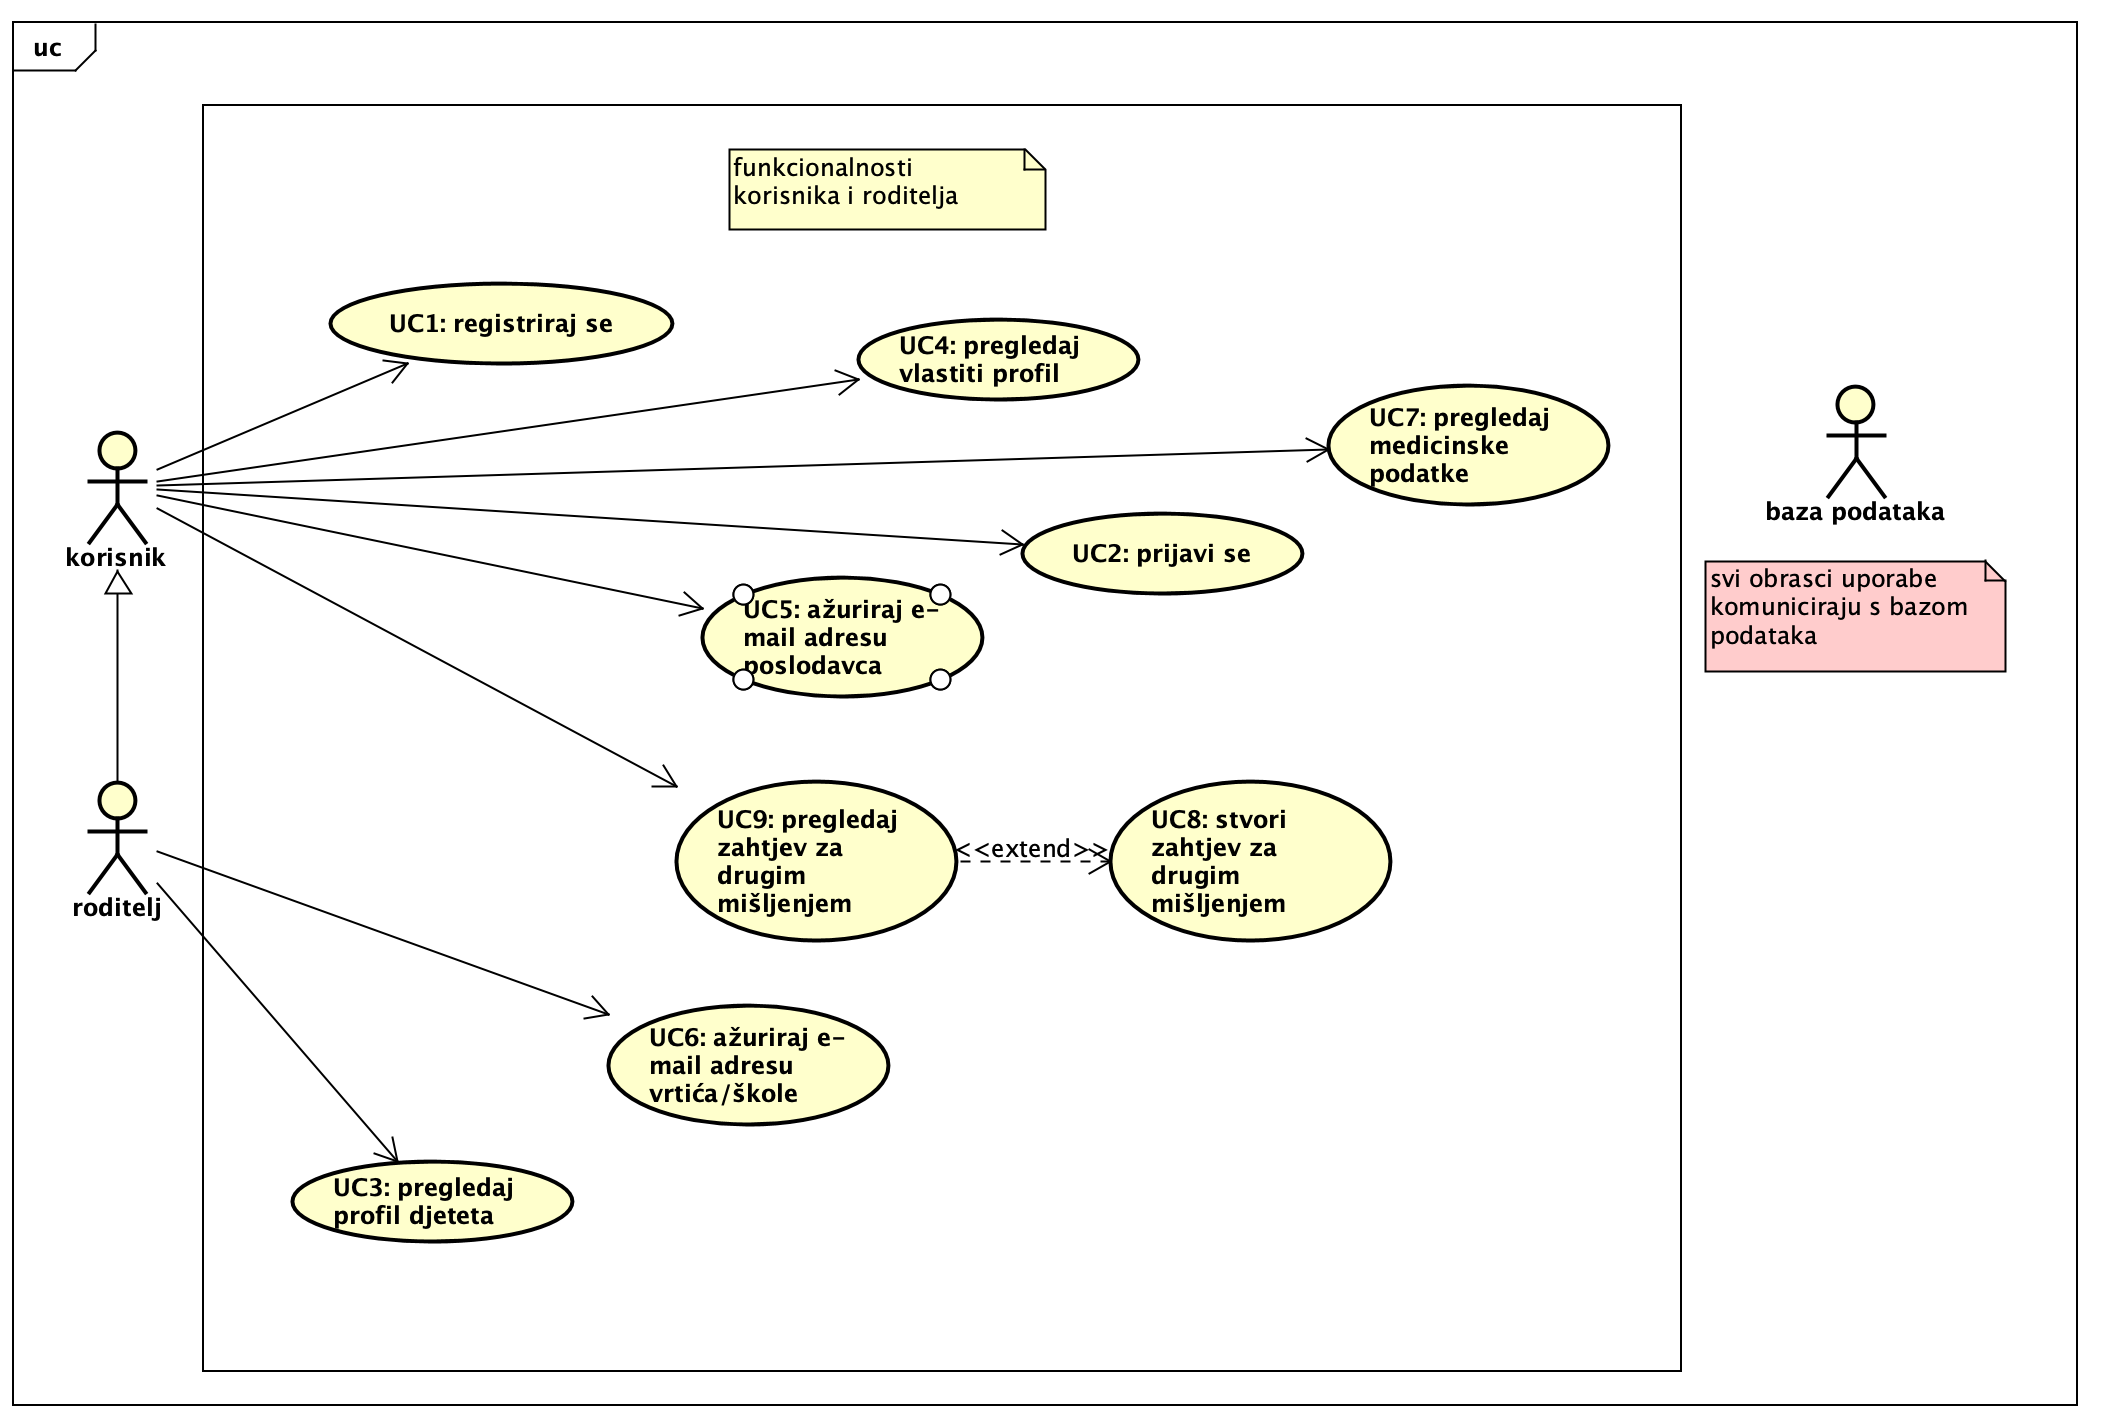
\includegraphics[width=\textwidth]{slike/uc_korisnik.png} 
						\caption{Dijagram obrasca uporabe, funkcionalnosti korisnika i roditelja}
					\end{figure}
					\begin{figure}[H]
						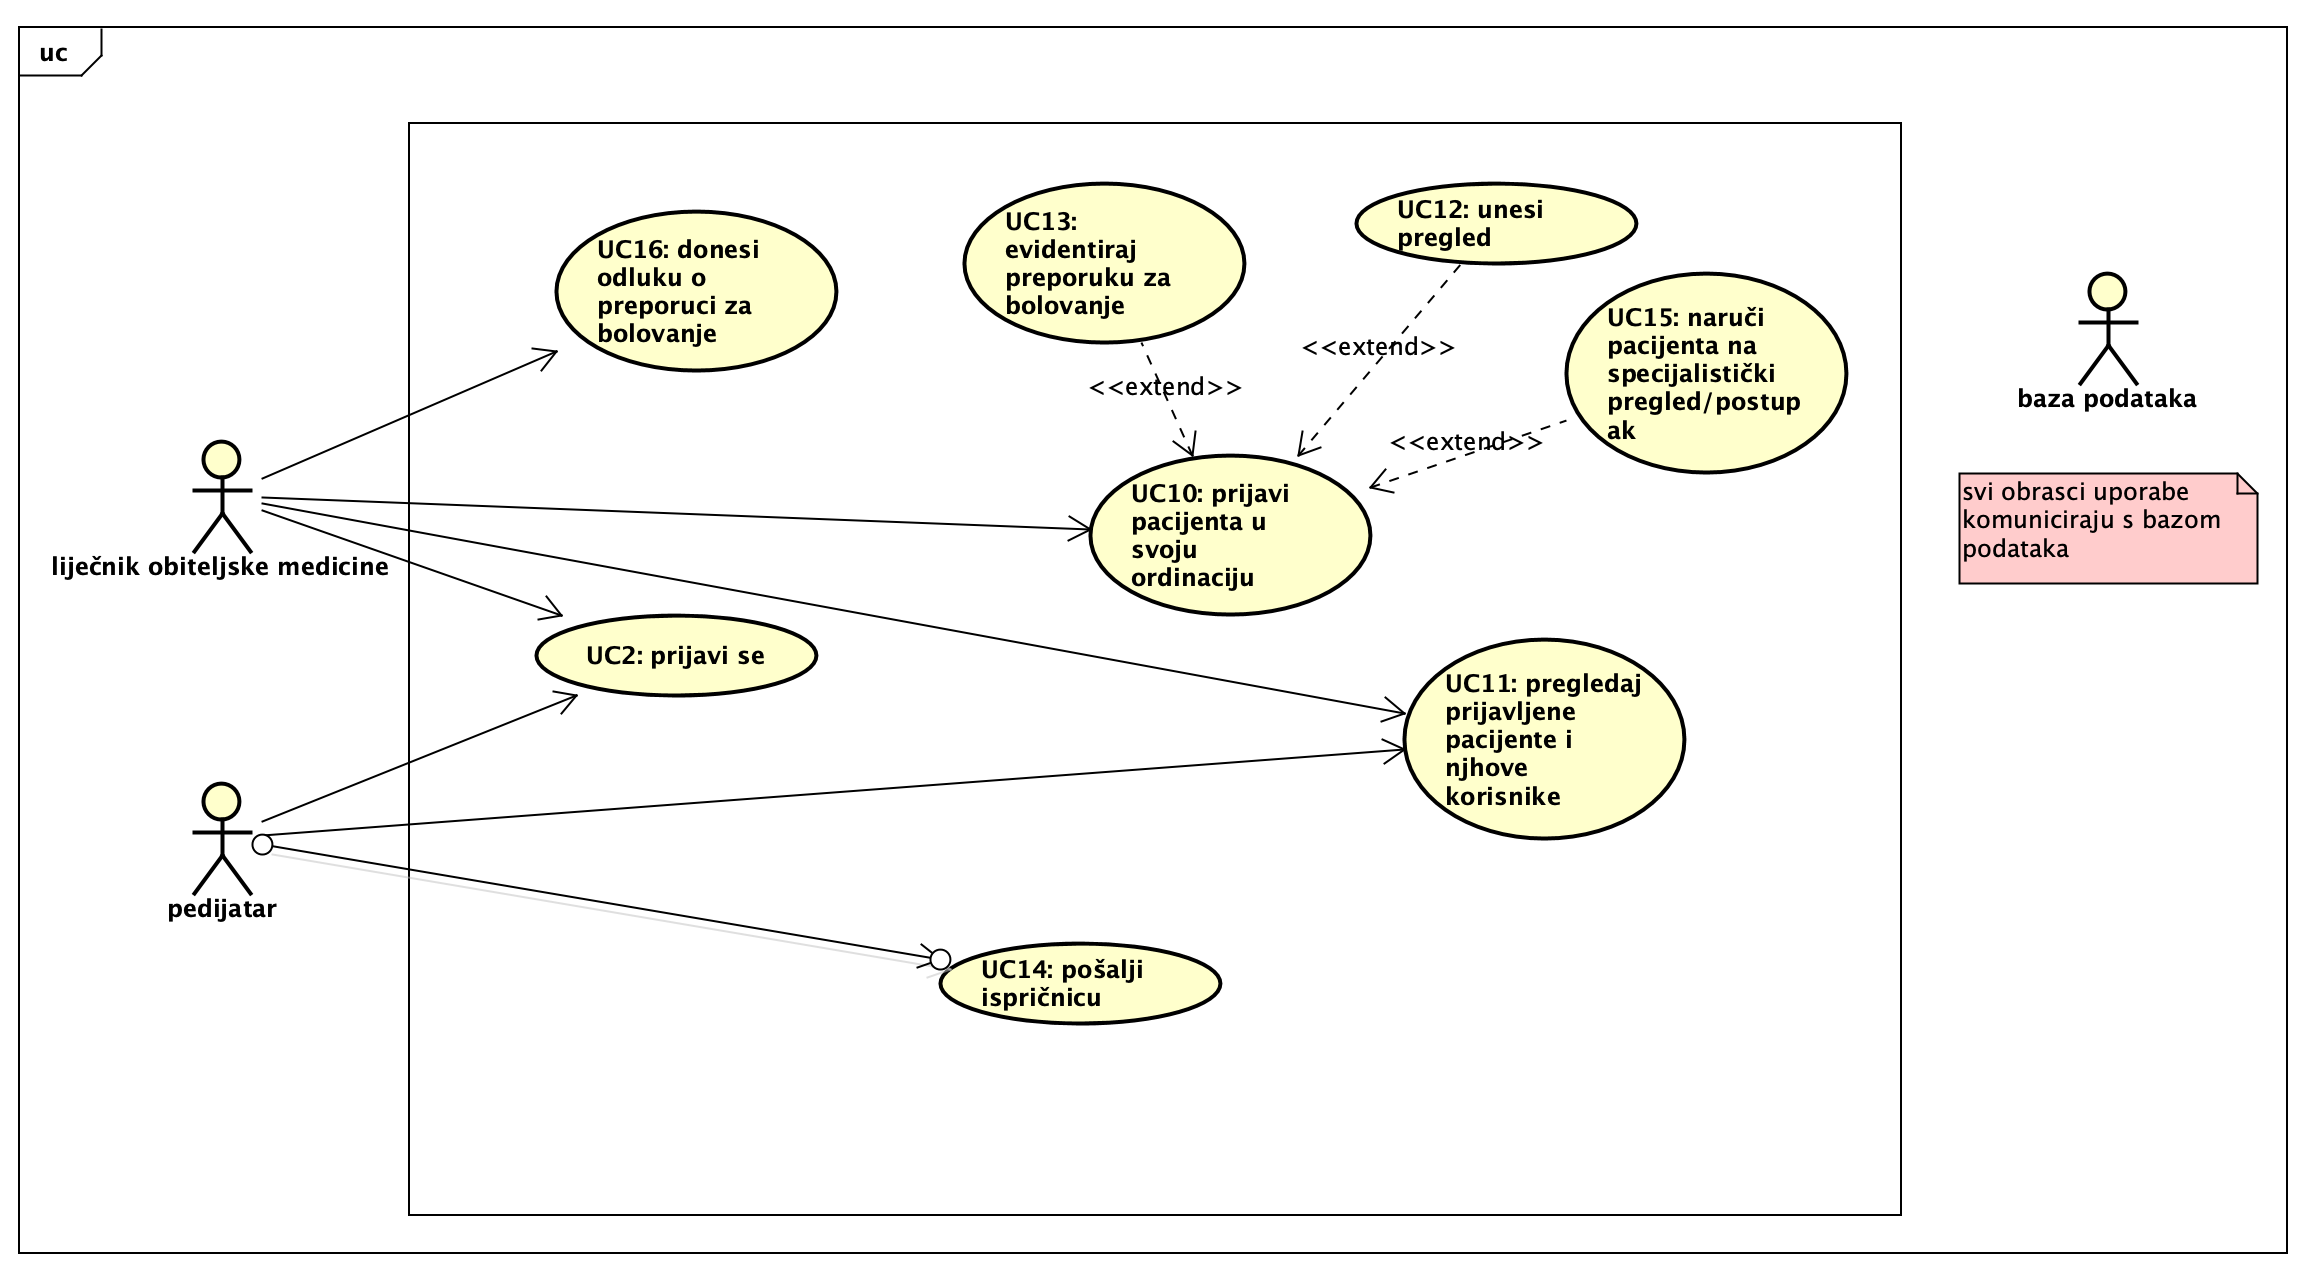
\includegraphics[width=\textwidth]{slike/uc_dr.png} 
						\caption{Dijagram obrasca uporabe, funkcionalnosti liječnika obiteljske medicine i pedijatra}
					\end{figure}
					\begin{figure}[H]
						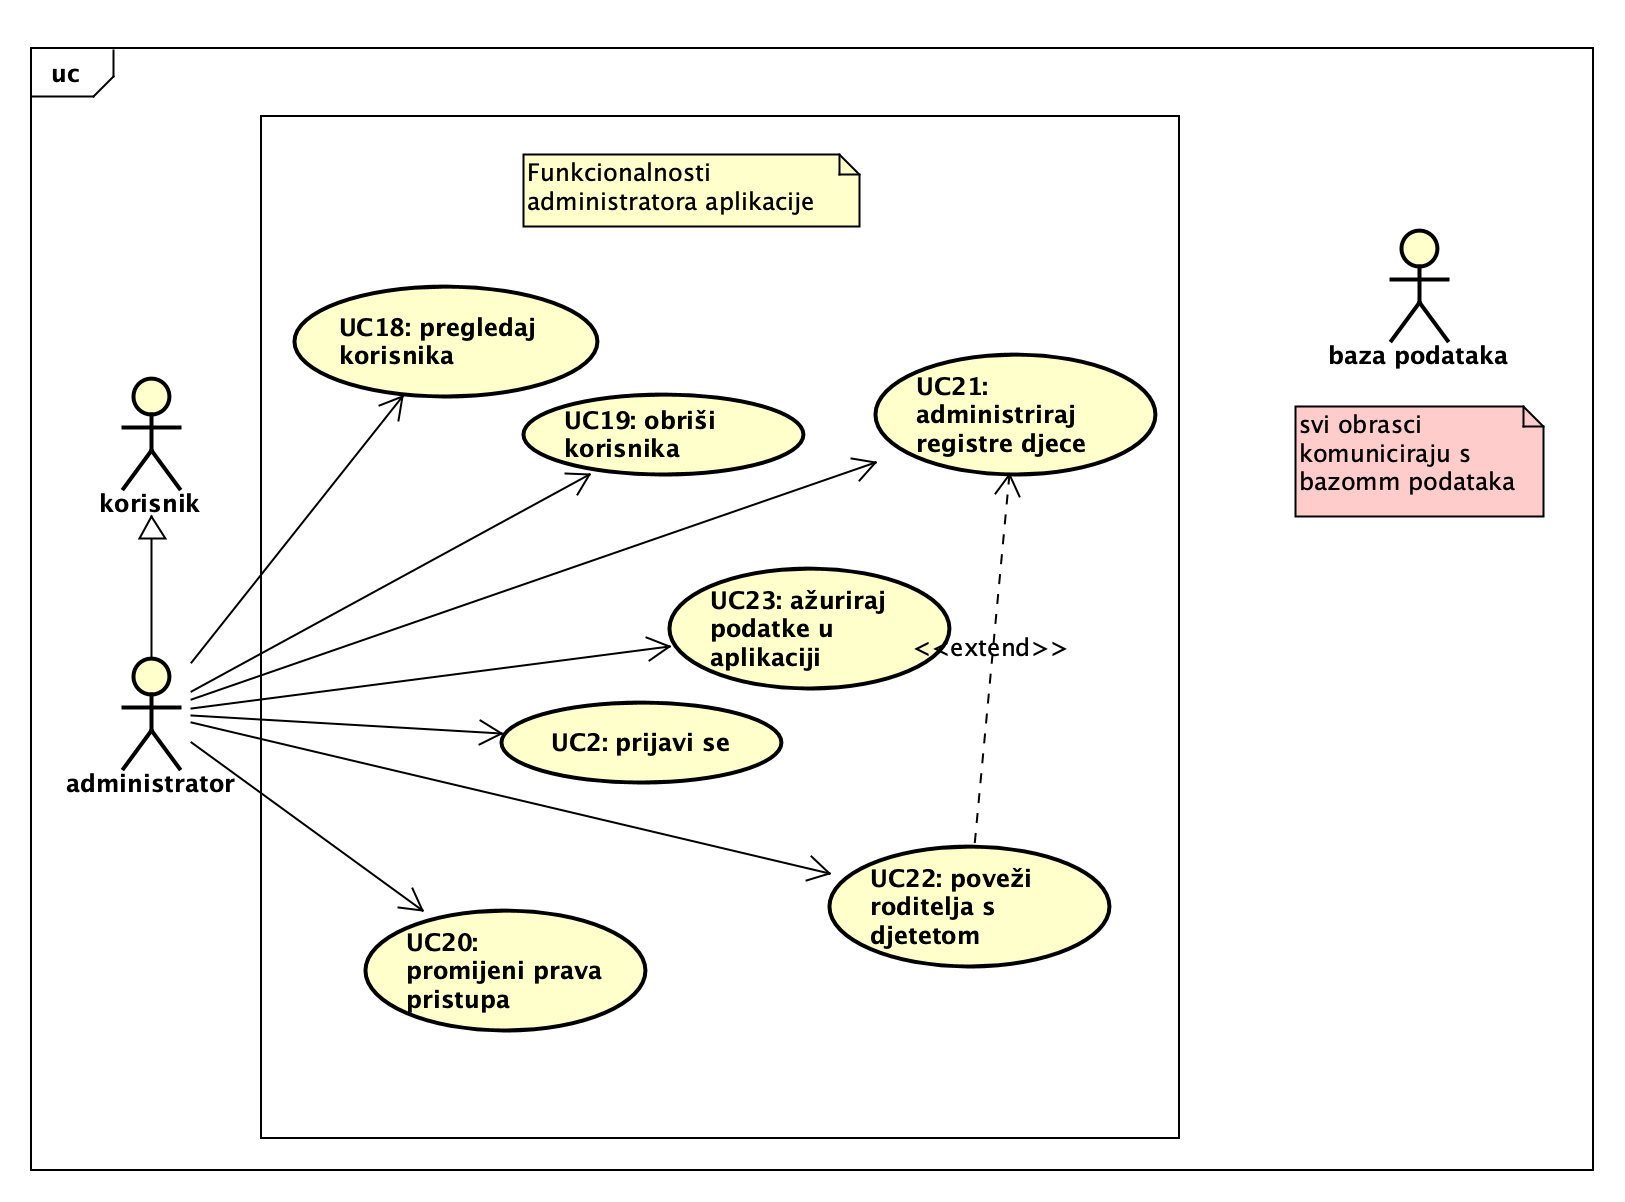
\includegraphics[width=\textwidth]{slike/uc_admin.png} 
						\caption{Dijagram obrasca uporabe, funkcionalnosti administratora}
					\end{figure}
				\eject		
				
			\subsection{Sekvencijski dijagrami}
				\subsubsection*{Obrazac uporabe UC9 - stvori zahtjev za drugim mišljenjem}
				Kroz proces potraživanja drugog mišljenja, korisnik inicira postupak odabirom opcije 
				'Zatraži drugo mišljenje'. Sustav odgovara otvaranjem modalnog okvira za unos zahtjeva, 
				gdje korisnik, u ovom slučaju roditelj, prenosi medicinski nalaz. Nakon toga, korisnik 
				bira specifičnog liječnika ili pedijatra čije drugo mišljenje želi dobiti i potvrđuje 
				zahtjev odabirom akcije 'Pošalji zahtjev'. Sustav potom provjerava i potvrđuje valjanost 
				unosa, prikazujući korisniku poruku o uspješnom slanju zahtjeva. U slučaju neispravno 
				popunjenog zahtjeva, sustav usmjerava korisnika na ponovni unos, osiguravajući točnost 
				informacija prije nastavka postupka. \\

				\begin{figure}[H]
						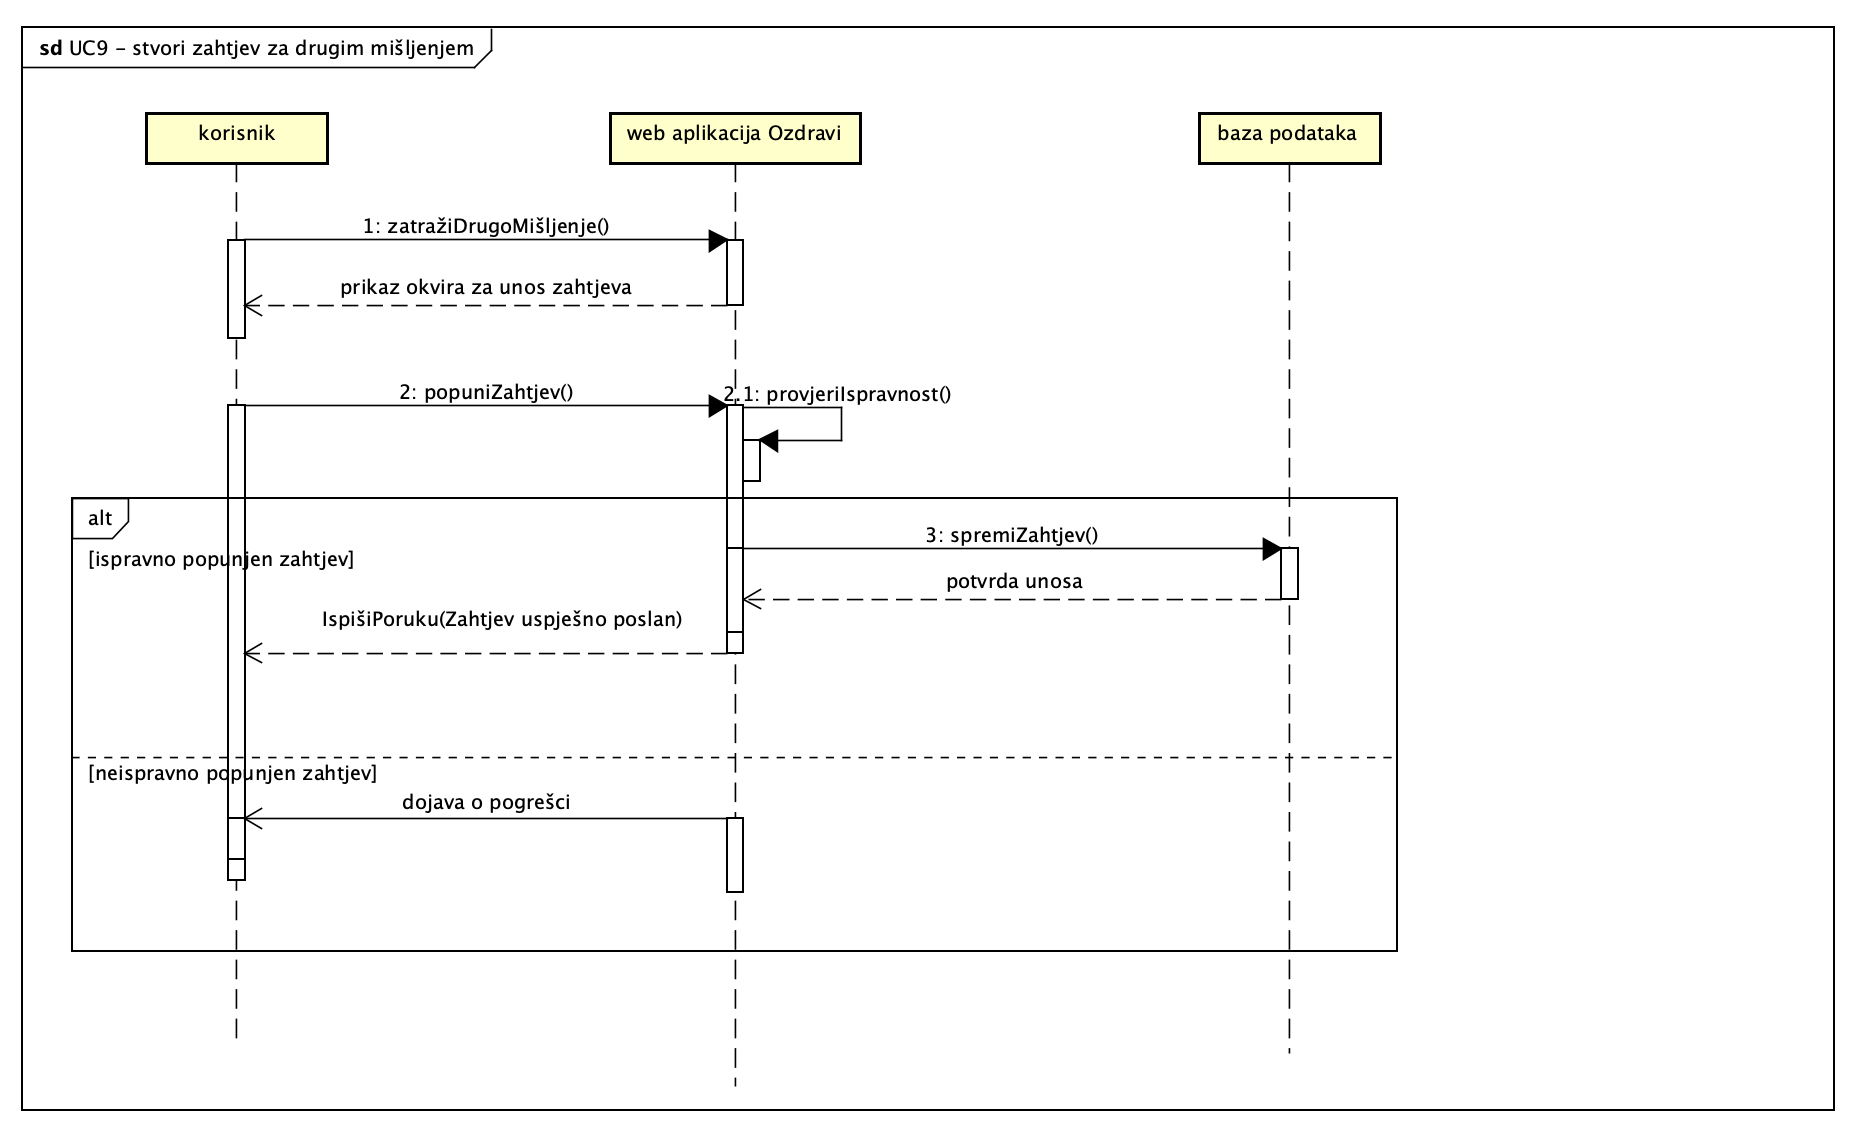
\includegraphics[width=\textwidth]{slike/sduc9.png} 
						\caption{Sekvencijski dijagram za UC9}
				\end{figure}
				\eject

				\subsubsection*{Obrazac uporabe UC14 - evidentiraj preporuku za bolovanje}
				U postupku stvaranja nove preporuke za bolovanje, pedijatar započinje odabirom opcije 'Preporuke za bolovanje'.
				Zatim odabire opciju 'Nova preporuka za bolovanje'. Sustav reagira prikazivanjem modalnog 
				okvira za unos preporuke za bolovanje. Pedijatar zatim odabire pregled na temelju kojeg 
				je potrebna preporuka za bolovanje i unosi relevantne podatke o preporuci. Kada završi 
				s unosom, pedijatar odabire opciju 'Unesi preporuku'. Sustav provjerava i potvrđuje 
				uspješan unos, nakon čega obavještava pedijatra o uspješnom dodavanju preporuke. \\

				\begin{figure}[H]
						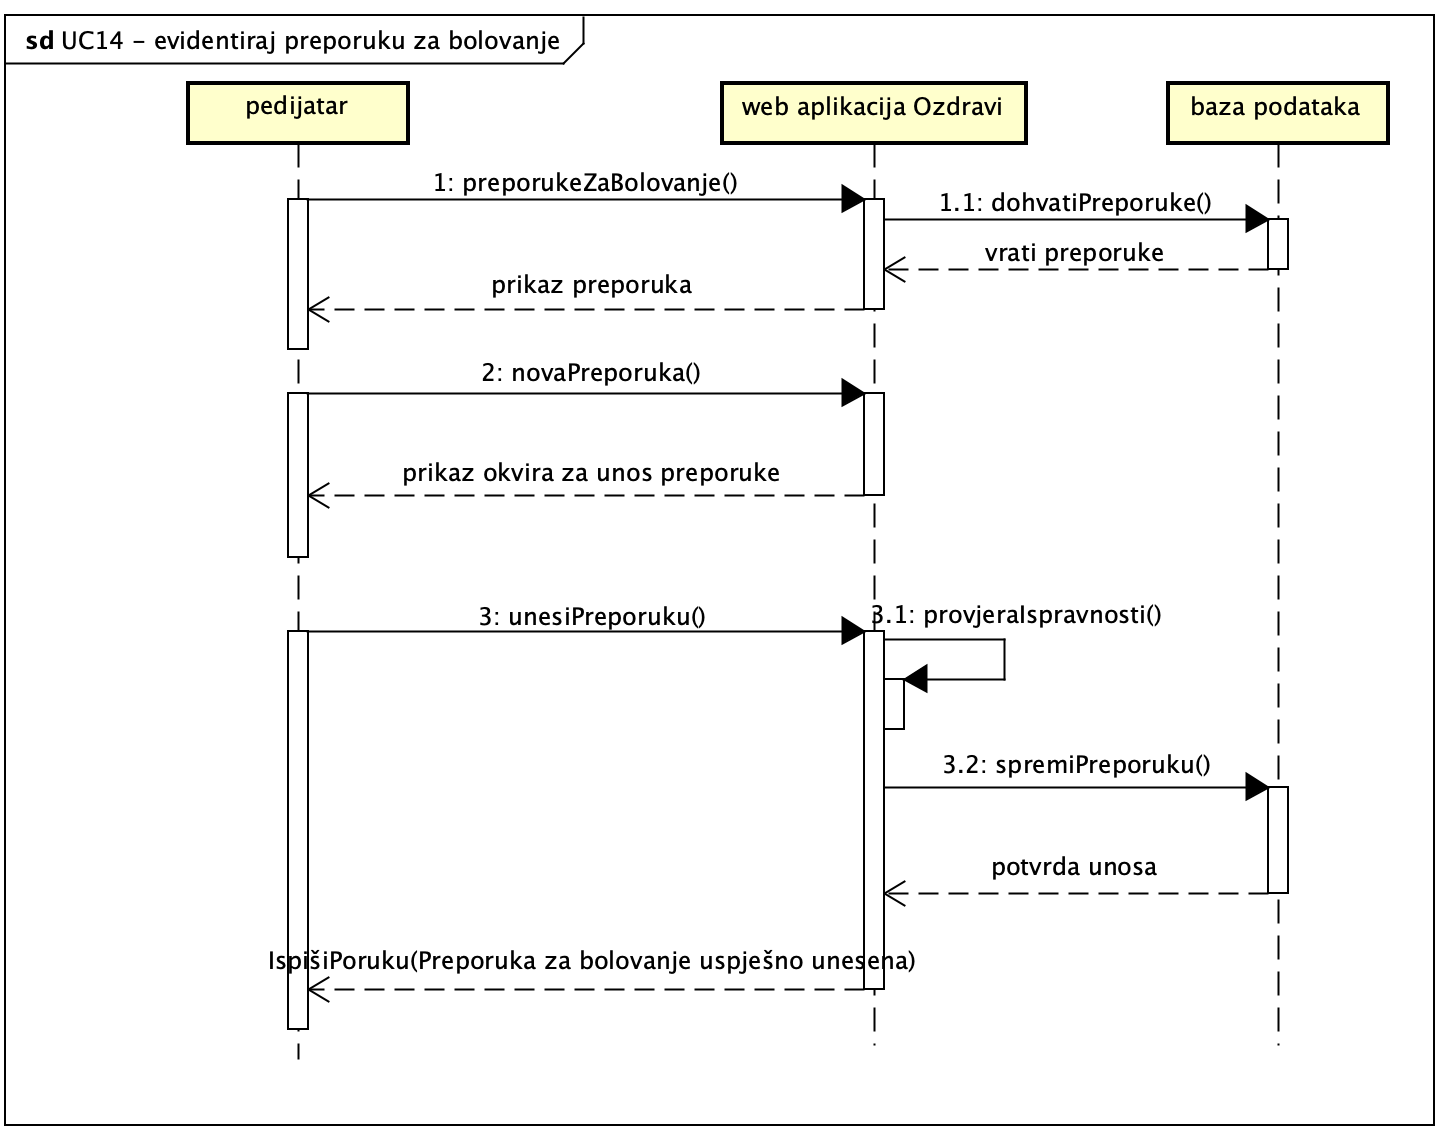
\includegraphics[width=\textwidth]{slike/sduc14.png} 
						\caption{Sekvencijski dijagram za UC14}
				\end{figure}
				\eject
				
				\subsubsection*{Obrazac uporabe UC15 - pošalji ispričnicu u vrtić/školu}

				U procesu izdavanja nove ispričnice, pedijatar započinje odabirom opcije 'Pregledi' 
				na početnoj stranici, što pokreće sustav da prikaže popis svih obavljenih pregleda. 
				Pedijatar tada odabire pregled na temelju kojeg je potrebno poslati ispričnicu. Na modalnom ekranu pregleda pedijatar bira opciju 
				'Pošalji ispričnicu' i na novom modalnom ekranu unosi tekst ispričnice. Nakon toga, bira opciju 'Spremi'.
				Sustav izvršava provjeru i potvrđuje uspješan unos, nakon čega obavještava pedijatra da je 
				ispričnica uspješno poslana. U slučaju neispravnog popunjavanja ispričnice, sustav 
				prikazuje poruku o neispravnom unosu podataka, a pedijatar se vraća na ponovno 
				popunjavanje ispričnice. \\

				\begin{figure}[H]
						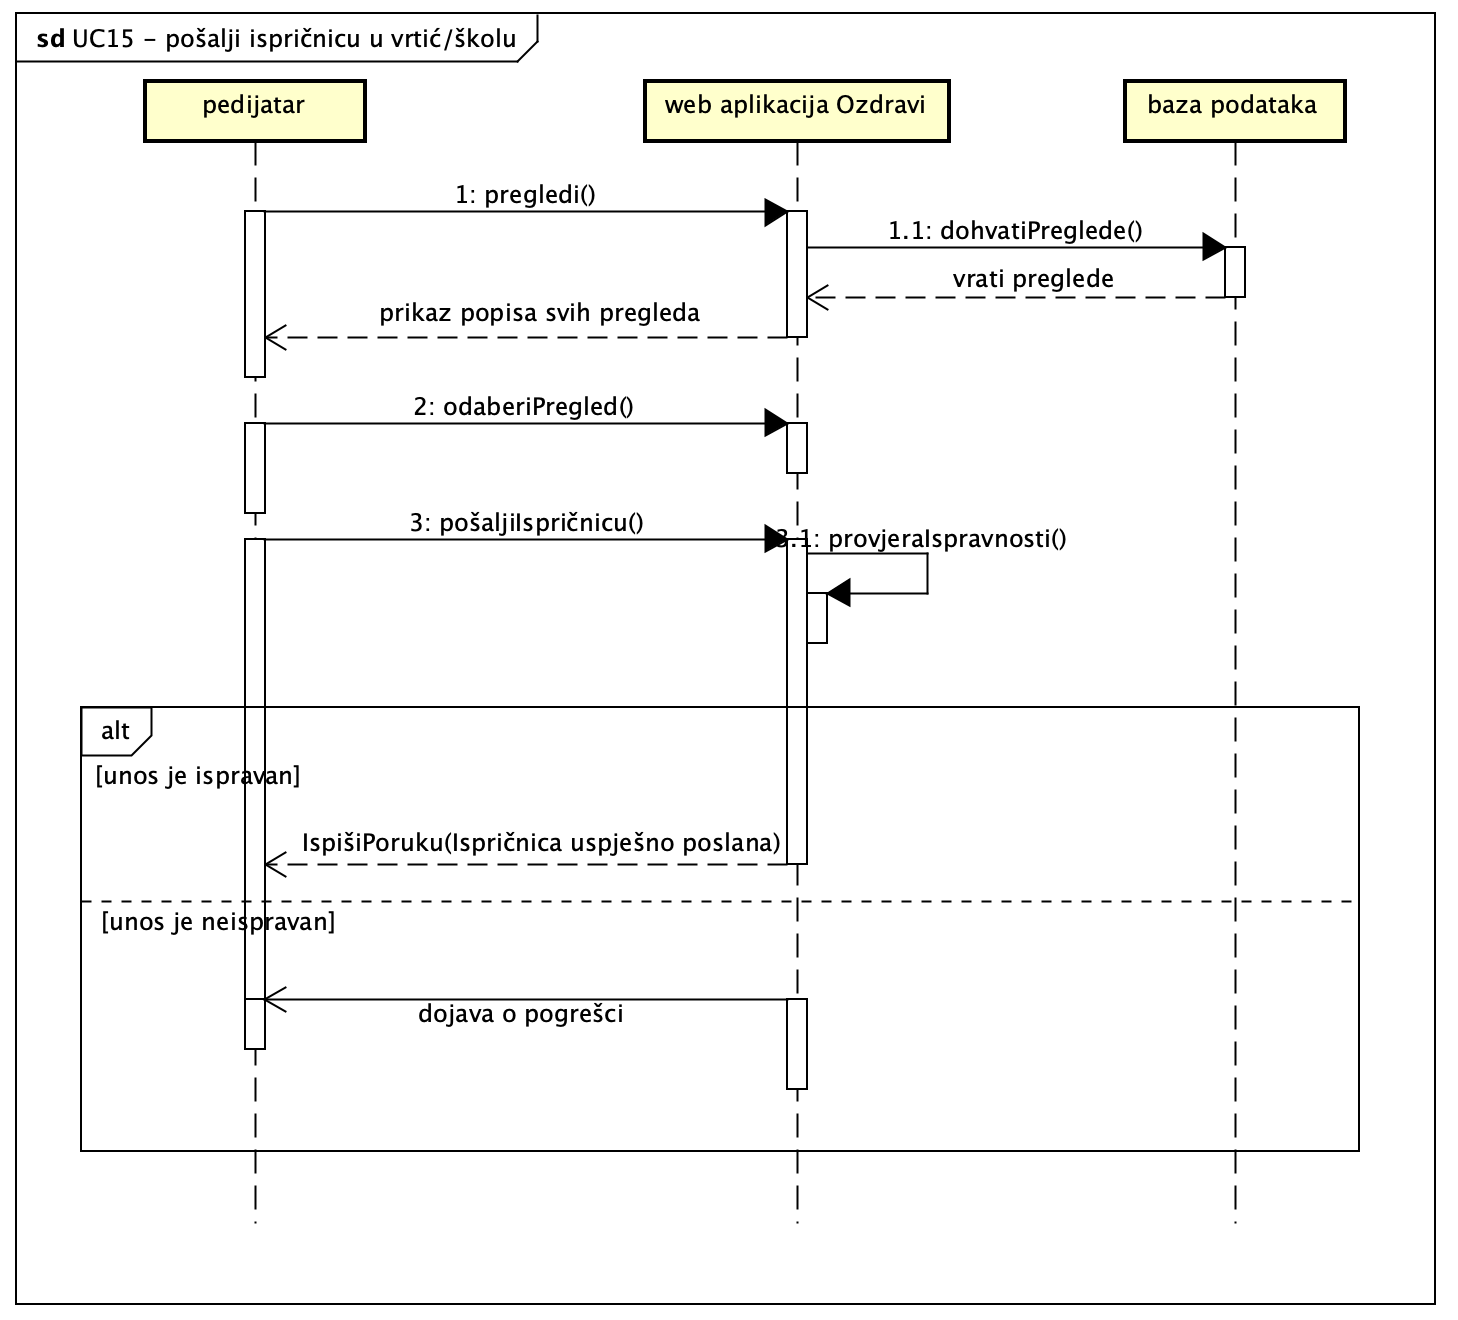
\includegraphics[width=\textwidth]{slike/sduc15.png} 
						\caption{Sekvencijski dijagram za UC15}
				\end{figure}

				\eject


	
		\section{Ostali zahtjevi}
			%dio 1. revizije
			 %Nefunkcionalni zahtjevi i zahtjevi domene primjene dopunjuju funkcionalne zahtjeve. Oni opisuju kako se sustav treba ponašati i koja ograničenja treba poštivati (performanse, korisničko iskustvo, pouzdanost, standardi kvalitete, sigurnost...). Primjeri takvih zahtjeva u Vašem projektu mogu biti: podržani jezici korisničkog sučelja, vrijeme odziva, najveći mogući podržani broj korisnika, podržane web/mobilne platforme, razina zaštite (protokoli komunikacije, kriptiranje...)... Svaki takav zahtjev potrebno je navesti u jednoj ili dvije rečenice.
			 \begin{packed_item}
				\item Sustav treba omogućiti rad više korisnika u stvarnom vremenu
				\item Sustav treba pružati brz odziv na korisničke zahtjeve
				\item Korisničko sučelje i sustav moraju podržavati hrvatsku abecedu (dijakritičke znakove) pri unosu i prikazu tekstualnog sadržaja
				\item Izvršavanje dijela programa u kojem se pristupa bazi podataka ne smije trajati duže od nekoliko sekundi
				\item Sustav treba biti implementiran kao web aplikacija koristeći objektno-orijentirane jezike
				\item Neispravno korištenje korisničkog sučelja ne smije narušiti funkcionalnost i rad sustava
				\item Sustav treba biti jednostavan za korištenje, sučelje treba biti intuitivno te se korisnici moraju znati koristiti sučeljem bez opširnih uputa
				\item Veza s bazom podataka mora biti kvalitetno zaštićena, brza i otporna na vanjske greške
				\item Pristup sustavu mora biti omogućen iz javne mreže koristeći HTTPS protokol
				\item Svi osjetljivi korisnički podaci, uključujući medicinske informacije, moraju biti kriptirani u 
				prijenosu i pohranjeni na način koji udovoljava standardima sigurnosti podataka u zdravstvenim aplikacijama
			 \end{packed_item}
			 	 
			 
	